\documentclass[12pt]{beamer}
\usepackage[utf8]{inputenc}
\usepackage[main=ukrainian,english]{babel}
\usepackage{amsmath}
\usetheme{Berkeley}
\logo{
\includegraphics[height=1.5cm]{images/Lviv_Polytechnic} }

\title{Усунення шуму на зображеннях}
\author{Ольга Павлюк, Роман Кутельмах}
\subtitle{{ дослідження,  розроблення алгоритмів та програмного забезпечення}}
\institute{Національний університет "Львівська політехніка", кафедра ПЗ}

\date{\today}

\begin{document}

\begin{frame}
	\titlepage
\end{frame}

\begin{frame}
	\frametitle{Зміст} 
	\tableofcontents
\end{frame}

\section{Проблема шуму в зображеннях}
\subsection{Визначення}
\begin{frame}\frametitle{Проблема шуму на зображеннях}
	\begin{block}{Шум}
	випадкові, відсутні на реальному зображенні відхилення інтенсивності
	\end{block}
	\linebreak
	Поширена проблема для цифрових зображень у багатьох галузях.\linebreak
	Виникає при недостатьому освітленні та високій ISO камери. 
	
	\begin{block}{Формальний опис}
		v(i) = u(i) + n(i), де i - піксель зображення \linebreak
		v(i) - спостережене значення, u(i) - справжнє значення \linebreak
		n(i) - значення шуму 
	\end{block}
\end{frame}

\subsection{Характеристики}
\begin{frame}\frametitle{Параметри оцінки алгоритмів}
	\begin{enumerate}
		\item автоматичні: PSNR
		
		\item візуальна оцінка
	\end{enumerate}
\end{frame}

\subsection{Методи вирішення}
\begin{frame}\frametitle{Існуючі підходи до усунення шуму}
	\begin{enumerate}
		\item просторові\pause
		\item частотні
	\end{enumerate}
\end{frame}


\section{Завдання магістерського дослідження}
\begin{frame}\frametitle{Завдання магістерського дослідження}
	\begin{block}{Об'єкт}
		шум на зображеннях
	\end{block}
	\begin{block}{Предмет}
			алгоритм для усунення шуму
	\end{block}
	\begin{block}{Мета}
		імплементувати чоткий алгоритм, \newline підібрати параметри,\newline  застосувати ліпші методи інтерполяції
	\end{block}
\end{frame}

\begin{frame}\frametitle{наукова новизна}
	імплементувати curvelet trasnform та дослідити кількість рівнів tiling grid, найліпші вейвлети тощо
\end{frame}

\section{Алгоритм Curvelet Transform}
\begin{frame}\frametitle{Алгоритм Curvelet Transform }
\end{frame}

\begin{frame}\frametitle{Перетворення Фур'є (Fourier Transform)  }
\end{frame}

\begin{frame}\frametitle{Перетворення Радона (Radon Transform) }
\end{frame}

\begin{frame}\frametitle{Project-Slice Theorem }
\end{frame}

\begin{frame}\frametitle{Ridglet Transform }
\end{frame}

\begin{frame}\frametitle{Frequency Grid Tiling }
\end{frame}

\section{Використані технології}
\begin{frame}\frametitle{Використані технології: C++ та OpenGL}
	Переваги:
	\begin{enumerate}
		\item C++: швидкість обчислень  + гнучка архітектура
		\item GLSL: обчислення на GPU в десятки разів швидше  
	\end{enumerate}
	Недоліки:
	\begin{enumerate}
		\item GLSL: труднощі у відлагодженні програм
	\end{enumerate}

	Приклад коду шейдера:
	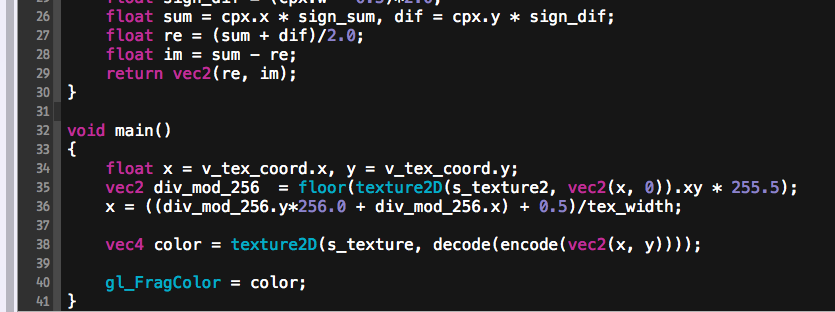
\includegraphics[height=2.5cm]{images/shader_snapshot}
\end{frame}

\subsection{Архітектура: діаграма класів проекту}
\begin{frame}\frametitle{Діаграма класів Curvelet Transform}
	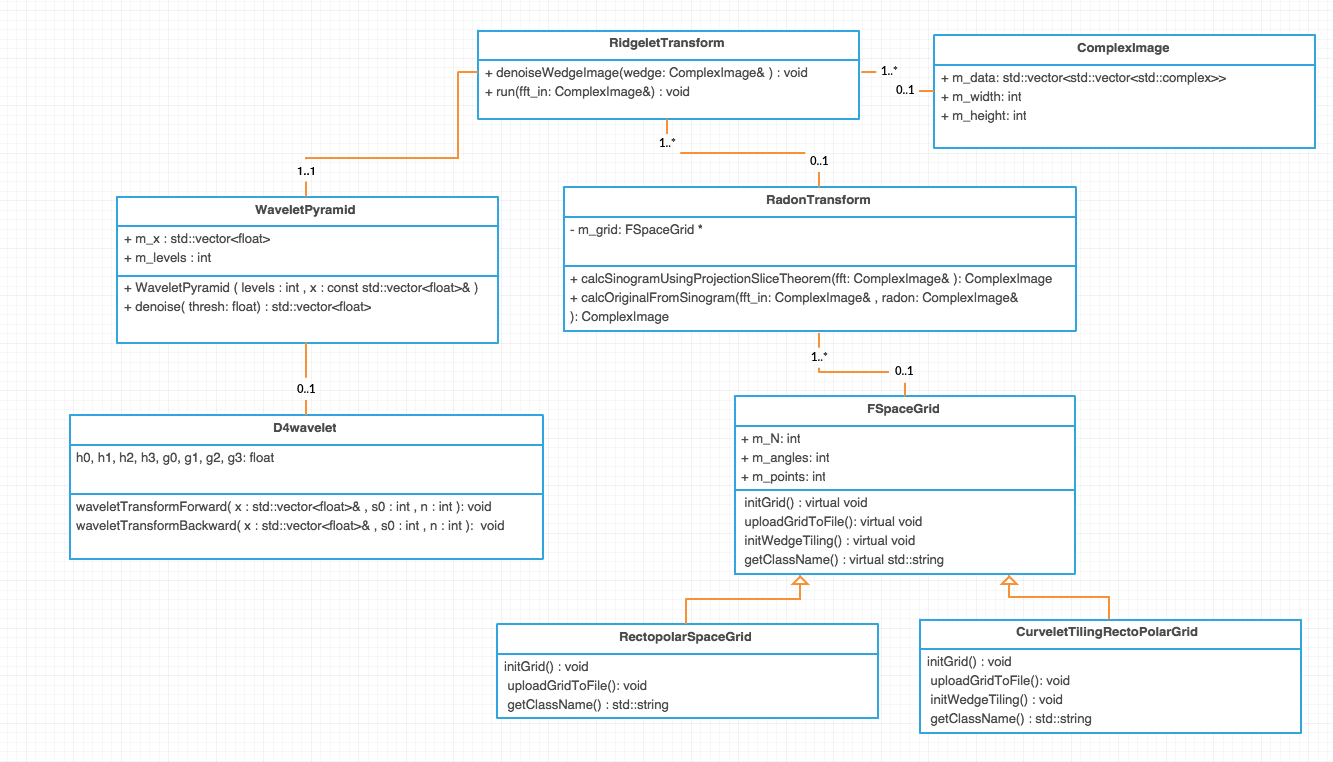
\includegraphics[scale=0.2]{images/class_diagram}
\end{frame}

\section{Поточні результати}
\begin{frame}\frametitle{Поточні результати}
	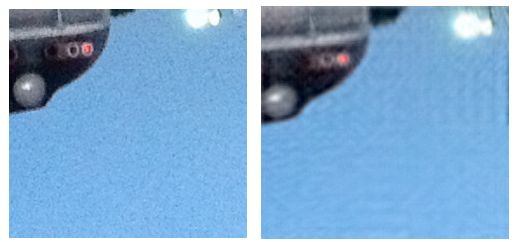
\includegraphics[height=3.5cm]{images/res_algo_1} \newline
	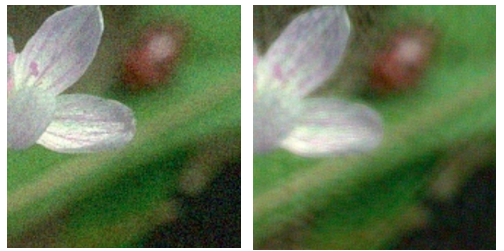
\includegraphics[height=3cm]{images/res_algo_2}
\end{frame}

\section{Висновки}
\begin{frame}\frametitle{Висновки }
	curvelet transform - good choise \newline
	никто не уйдет от покращення
\end{frame}

\begin{frame}\frametitle{}
	Дякую за увагу!
\end{frame}


\end{document}
